\documentclass[tikz,border=4pt]{standalone}
% Paleta y fuentes compartidas por el libro y las figuras (única fuente de verdad).
\RequirePackage{xcolor}
\definecolor{oxido}{HTML}{B7410E}
\definecolor{cobre}{HTML}{D27D2D}
\definecolor{carbon}{HTML}{2B2B2B}
\definecolor{azul}{HTML}{1F5F8B}
\definecolor{arena}{HTML}{F4EDE4}

\usepackage{fontspec}
\setsansfont{FiraSans}[Extension=.otf,UprightFont=*-Regular,BoldFont=*-SemiBold,ItalicFont=*-Italic,BoldItalicFont=*-SemiBoldItalic]
\setmonofont{FiraMono}[Extension=.otf,UprightFont=*-Regular,BoldFont=*-Medium,Scale=0.95]
\usetikzlibrary{positioning,arrows.meta,calc}
\begin{document}
\sffamily\small
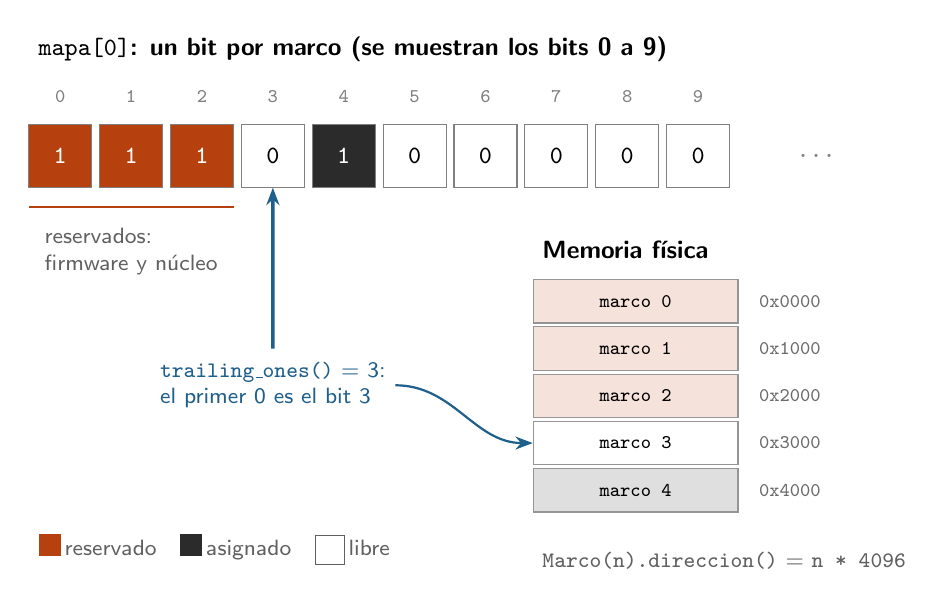
\begin{tikzpicture}[>={Stealth[length=2.2mm]},
  execute at begin node={\hyphenpenalty=10000},
  bit/.style={draw=carbon!60,minimum width=8mm,minimum height=8mm,
    inner sep=0pt,font=\ttfamily\small},
  nota/.style={font=\sffamily\footnotesize,text=carbon!75,align=left}]
  % Índices de bit (se muestran los bits 0 a 9 de mapa[0])
  \node[font=\sffamily\small\bfseries,anchor=west] at (-0.4,1.35) {\texttt{mapa[0]}: un bit por marco (se muestran los bits 0 a 9)};
  \foreach \i in {0,...,9} {
    \node[font=\ttfamily\scriptsize,text=carbon!60] at (\i*0.9,0.75) {\i};
  }
  \foreach \i/\v/\c in {0/1/oxido,1/1/oxido,2/1/oxido,3/0/white,4/1/carbon,5/0/white,6/0/white,7/0/white,8/0/white,9/0/white} {
    \ifnum\v=1
      \node[bit,fill=\c,text=white] (b\i) at (\i*0.9,0) {\v};
    \else
      \node[bit,fill=white] (b\i) at (\i*0.9,0) {\v};
    \fi
  }
  \node[font=\ttfamily\small,text=carbon!60] at (9.6,0) {\dots};
  % Llave de los reservados
  \draw[oxido,thick] (-0.4,-0.65) -- (2.2,-0.65);
  \node[nota,anchor=north] at (0.9,-0.8) {reservados:\\firmware y núcleo};
  % trailing_ones
  \draw[->,azul,very thick] (2.7,-2.45) -- (b3.south);
  \node[nota,anchor=north,text=azul] (to) at (2.7,-2.5) {\texttt{trailing\_ones()} = 3:\\el primer 0 es el bit 3};
  % Correspondencia con memoria física
  \node[font=\sffamily\small\bfseries,anchor=west] at (6.0,-1.2) {Memoria física};
  \foreach \i/\d/\c in {0/0x0000/oxido!15,1/0x1000/oxido!15,2/0x2000/oxido!15,3/0x3000/white,4/0x4000/carbon!15} {
    \node[draw=carbon!50,fill=\c,
      minimum width=26mm,minimum height=5.5mm,font=\ttfamily\scriptsize,anchor=west]
      (m\i) at (6.0,-1.85-\i*0.6) {marco \i};
    \node[font=\ttfamily\scriptsize,text=carbon!70,anchor=west] at (8.75,-1.85-\i*0.6) {\d};
  }
  \draw[->,azul,thick] (to.east) to[out=0,in=180] (m3.west);
  % Leyenda
  \node[nota,anchor=west] at (-0.4,-5.0) {\textcolor{oxido}{\rule{8pt}{8pt}}\,reservado\quad
    \textcolor{carbon}{\rule{8pt}{8pt}}\,asignado\quad
    \fbox{\rule{0pt}{4pt}\hspace{4pt}}\,libre};
  \node[nota,anchor=west] at (6.0,-5.15) {\texttt{Marco(n).direccion()} = \texttt{n * 4096}};
\end{tikzpicture}
\end{document}
